%!TeX root = BasiDiDati.tex

\chapter{Linguaggio SQL}
Il termine SQL in origine era l'acronimo di \textbf{S}tructured \textbf{Q}uery \textbf{L}anguage, ma ad oggi è diventato un nome proprio.

\definizione{linguaggio SQL}{
  \raggedright
  Il \textbf{linguaggio di interrogazione SQL} permette di:
  \begin{itemize}[label=$\triangleright$, itemsep=\smallskipamount]
    \item \textbf{definire delle strutture dati e i vincoli di integrità}: \textcolor{azzurrino}{\textbf{D}}ata \textcolor{azzurrino}{\textbf{D}}efinition \textcolor{azzurrino}{\textbf{L}}anguage
    \item \textbf{manipolare i dati} (inserimento, aggiornamento e cancellazione): \textcolor{azzurrino}{\textbf{D}}ata \textcolor{azzurrino}{\textbf{M}}anipilation \textcolor{azzurrino}{\textbf{L}}anguage
    \item \textbf{interrogare}: \textcolor{azzurrino}{\textbf{D}}ata \textcolor{azzurrino}{\textbf{Q}}uery \textcolor{azzurrino}{\textbf{L}}anguage
  \end{itemize}
}

Esistono diverse versioni:

\begin{center}
  \begin{longtable}{|c|c|l|}
  \hline
  \textbf{Nome informale} & \textbf{Nome ufficiale} & \multicolumn{1}{c|}{\textbf{Caratteristiche}} \\ \hline
  \endfirsthead
  \hline
  \textbf{Nome informale} & \textbf{Nome ufficiale} & \multicolumn{1}{c|}{\textbf{Caratteristiche}} \\ \hline
  \endhead

  \multirow{2}{*}{SQL base} & SQL-86 & Costrutti base \\ \cline{2-3} 
                            & SQL-89 & Integrità referenziale \\ \hline
  SQL-2                     & SQL-92 & \begin{tabular}[c]{@{}l@{}}Modello relazionale\\ Vari costrutti nuovi\\ 3 livelli: entry, intermediate, full\end{tabular} \\ \hline
  \multirow{10}{*}{SQL-3}   & SQL:1999 & \begin{tabular}[c]{@{}l@{}}Modello relazionale a oggetti\\ Organizzato in diverse parti\\ Trigger, funzioni esterne, ...\end{tabular} \\ \cline{2-3} 
                            & SQL:2003 & \begin{tabular}[c]{@{}l@{}}Estensioni del modello a oggetti\\ Eliminazione di costrutti non usati\\ Nuove parti: SQL/JRT, SQL/XML, ...\end{tabular} \\ \cline{2-3} 
                            & SQL:2006 & Estensione della parte XML \\ \cline{2-3} 
                            & SQL:2008 & Lievi aggiunte (per esempio, \texttt{trigger instead of}) \\ \cline{2-3} 
                            & SQL:2011 & Ricco supporto per dati temporali \\ \cline{2-3} 
                            & SQL:2016 & Gestione del formato JSON \\ \hline
  \end{longtable}
\end{center}

La parte di SQL dedicata alle dichiarazioni fa parte dei DML.\\[0.2ex]
\hl{Le dichiarazioni vengono espresse in modo dichiarativo}: viene specificato l'obiettivo e non la procedura per ottenerlo (algebra relazionale).

Una parte del DBMS, detta $\verb|query optimizer|$, traduce l’interrogazione SQL nel linguaggio procedurale interno del sistema, che è nascosto all’utente.\\[0.2ex]
SQL permette, quindi, di descrivere le interrogazioni in modo astratto e ad alto livello.

\section{Clausola \protect\texttt{SELECT}}
La sintassi dell’istruzione $\verb|SELECT|$ è:
\begin{lstlisting}[language=SQL]
SELECT [DISTINCT]
[ * | expression [[ AS ] output_name ] [, ...] ]
[ FROM from_item [, ...] ]
  [ WHERE condition ]
  [ GROUP BY grouping_element [, ...] ]
      [ HAVING condition [, ...] ]
      [ { UNION | INTERSECT | EXCEPT } [ DISTINCT ] other_select ]
        [ ORDER BY expression [ ASC | DESC | USING operator ] ]
\end{lstlisting}

dove:
\begin{itemize}[label=$\triangleright$, itemsep=\smallskipamount]
  \item $\verb|expression|$: espressione che determina un attributo
  \item $\verb|from_item|$: espressione che determina una sorgente per gli attributi
  \item $\verb|condition|$: espressione booleana per selezionare i valori degli attributi
  \item $\verb|grouping_element|$: espressione per poter eseguire operazioni su più valori di un attributo e considerare il risultato
\end{itemize}

\bigskip
La struttura dell’istruzione è la seguente:
\begin{lstlisting}[language=SQL]
SELECT attributo
FROM tabella
  [WHERE condizione]
\end{lstlisting}

$\verb|SELECT|$, $\verb|FROM|$ e $\verb|WHERE|$ sono chiamate \textcolor{azzurrino}{\textbf{clausole}}.

\medskip
La clausula $\verb|SELECT|$ estrae dal prodotto cartesiano delle tabelle,  elencate nella clausola $\verb|FROM|$, le righe che soddisfano la condizione specificata nella clausola $\verb|WHERE|$.\\[0.2ex]
Il risultato dell‘interrogazione è una tabella con una riga per ogni riga prodotta dalla clausola $\verb|FROM|$ ed, eventualmente, filtrata dalla clausola $\verb|WHERE|$, le cui colonne dipendono dalla lista degli attributi nella clausola $\verb|SELECT|$.

\begin{esempiobox}{Interrogazione con \texttt{SELECT}}
  Consideriamo la seguente base di dati:

  \smallskip
  \begin{center}
    \includegraphics[width=0.5\textwidth]{images/tabella-impiegato.png}
  \end{center}

  \smallskip
  $\boldsymbol{\mathrm{Q_1}}$\textbf{: estrarre lo stipendio degli impiegati di cognome 'Rossi'}

  \begin{lstlisting}[language=SQL]
  SELECT Stipendio
  FROM Impiegato
    WHERE Cognome = 'Rossi';
  \end{lstlisting}

  \smallskip
  Il risultato dell'interrogazione è la seguente tabella:
  \begin{center}
    \includegraphics[width=0.2\textwidth]{images/select-impiegato.png}
  \end{center}
\end{esempiobox}

\bigskip
Il simbolo $\verb|*|$ permette di  indicare tutti gli attributi delle tabelle.
\begin{lstlisting}[language=SQL]
SELECT *
FROM tabella;
\end{lstlisting}

\begin{esempiobox}{Interrogazione con \texttt{SELECT *}}
  Consideriamo la seguente tabella:

  \smallskip
  \begin{center}
    \includegraphics[width=0.5\textwidth]{images/tabella-impiegato.png}
  \end{center}

  \smallskip
  $\boldsymbol{\mathrm{Q_2}}$\textbf{: estrarre lo stipendio degli impiegati di cognome 'Rossi'}
  \begin{lstlisting}[language=SQL]
  SELECT *
  FROM Impiegato
    WHERE Cognome = 'Rossi';
  \end{lstlisting}

  \smallskip
  Il risultato dell'interrogazione è la seguente tabella:
  \begin{center}
    \includegraphics[width=0.6\textwidth]{images/select-all-impiegato.png}
  \end{center}
\end{esempiobox}

\section{Clasuola \protect\texttt{FROM}}
La clausola $\verb|FROM|$ specifica le tabelle da cui estrarre i dati.

La sintassi è:
\begin{lstlisting}[language=SQL]
FROM from_item [, ...]
\end{lstlisting}

dove $\verb|from_item|$ può essere una delle seguenti clausole:
\begin{itemize}[label=$\triangleright$, itemsep=\medskipamount]
  \item $\verb|table_name [[AS] alias [(column_alias [, ...])]]|$: se sono presenti due o più tabelle, si esegue il prodotto cartesiano tra tutte le tabelle. 
  
  Se ci sono attributi con lo stesso nome su tabelle diverse, nella $\verb|SELECT|$ questi attributi sono identificati anteponendo il nome della tabella e un ’.’ (es. $\verb|nomeTabella.nomeAttributo|$)
  \item $\verb|(other_select) [AS] nomeRisultato [(column_alias [,...])]|$: è una $\verb|SELECT|$ innestata. 
  
  Il risultato della $\verb|SELECT|$ interna è lo schema con nome $\verb|nomeRisultato|$ su cui fare la $\verb|SELECT|$ corrente.
  \item $\verb|from_item [NATURAL] join_type from_item [ON condition]|$: è la clausola JOIN. 
  
  Permette di selezionare un sottoinsieme del prodotto cartesiano di due o più tabelle. 
  
  $\verb|join_type|$ specifica il tipo di join
\end{itemize}

\begin{esempiobox}{Interrogazione con FROM}
  Consideriamo le seguenti tabelle:

  \smallskip
  \begin{center}
    \begin{minipage}{0.45\textwidth}
      \centering
      \includegraphics[width=\textwidth]{images/tabella-impiegato.png}
    \end{minipage}
    \hfill
    \begin{minipage}{0.45\textwidth}
      \centering
      \includegraphics[width=\textwidth]{images/tabella-dipartimento.png}
    \end{minipage}
  \end{center}

  \smallskip
  $\boldsymbol{\mathrm{Q_3}}$\textbf{: estrarre i nomi e il cognome degli impiegati e le città in cui lavorano}

  \begin{lstlisting}[language=SQL]
  SELECT Impiegato.Nome, Impiegato.Cognome, Dipartimento.Citta
  FROM Impiegato, Dipartimento
    WHERE Impiegato.Dipart = Dipartimento.Nome
  \end{lstlisting}

  \smallskip
  Il risultato dell'interrogazione è la seguente tabella:
  \begin{center}
    \includegraphics[width=0.4\textwidth]{images/from-impiegato-dipartimento.png}
  \end{center}
\end{esempiobox}

\section{Clausola \protect\texttt{WHERE}}
La sintassi è:

\begin{lstlisting}[language=SQL]
WHERE condition
\end{lstlisting}

La clausola $\verb|WHERE|$ ammette come argomento un’espressione booleana costruita combinando predicati semplici con gli operatori $\verb|AND|$, $\verb|OR|$ e $\verb|NOT|$:
\begin{itemize}[label=$\circ$, itemsep=\smallskipamount]
  \item \textbf{AND}: seleziona le righe in cui tutti i predicati sono veri
  \item \textbf{OR}: seleziona le righe in cui almeno un predicato è vero
  \item \textbf{NOT}: seleziona le righe in cui il predicato è falso
\end{itemize}

Ciascun predicato semplice usa gli operatori $\verb|=|$, $\verb|<>| (\verb|<>| \Leftrightarrow \neq)$, $\verb|<|$, $\verb|>|$, $\verb|<=|$, $\verb|>=|$ per confrontare un’espressione costruita a partire dal valore di un attributo con un valore costante, oppure un’altra espressione.

\begin{esempiobox}{Interrogazione con \texttt{WHERE}}
  Consideriamo le seguenti tabelle:

  \smallskip
  \begin{center}
    \begin{minipage}{0.45\textwidth}
      \centering
      \includegraphics[width=\textwidth]{images/tabella-impiegato.png}
    \end{minipage}
    \hfill
    \begin{minipage}{0.45\textwidth}
      \centering
      \includegraphics[width=\textwidth]{images/tabella-dipartimento.png}
    \end{minipage}
  \end{center}

  \smallskip
  $\boldsymbol{\mathrm{Q_4}}$\textbf{: estrarre i nomi e il cognome degli impiegati che lavorano nell'ufficio 20 del dipartimento Ammistrazione}
  \begin{lstlisting}[language=SQL]
  SELECT Nome, Cognome
  FROM Impiegato
    WHERE Ufficio = 20 AND Dipart = 'Amministrazione';
  \end{lstlisting}

  \smallskip
  Il risultato dell'interrrogazione è la seguente tabella:
  \begin{center}
    \includegraphics[width=0.3\textwidth]{images/where-impiegato-dipartimento.png}
  \end{center}
\end{esempiobox}

\subsection{Operatore \texttt{LIKE}}
Per il confronto tra stringhe, SQL mette a disposizione anche l’operatore $\verb|LIKE|$ che consente di verificare se una stringa rispetta un certo “pattern” (oppure $\verb|ILIKE|$ per \textbf{case insentive}).

I caratteri speciali per il confronto sono:
\begin{itemize}[label=$\diamond$, itemsep=\smallskipamount]
  \item \textbf{\_}: confronto con un carattere arbitrario
  \item \textbf{\%}: confronto con una stringa di lunghezza arbitraria (anche 0) di caratteri arbitrari
\end{itemize}

\begin{esempiobox}{Interrogazione con LIKE}
  Consideriamo le seguenti tabelle:

  \smallskip
  \begin{center}
    \begin{minipage}{0.45\textwidth}
      \centering
      \includegraphics[width=\textwidth]{images/tabella-impiegato.png}
    \end{minipage}
    \hfill
    \begin{minipage}{0.45\textwidth}
      \centering
      \includegraphics[width=\textwidth]{images/tabella-dipartimento.png}
    \end{minipage}
  \end{center}

  \smallskip
  $\boldsymbol{\mathrm{Q_5}}$\textbf{: estrarre gli impiegati che hanno un cognome che ha una "o" in seconda posizione e finisce con una "i"}
  \begin{lstlisting}[language=SQL]
  SELECT *
  FROM Impiegato
  WHERE Cogmome LIKE '_o%i'; 
  \end{lstlisting}

  \smallskip
  Il risultato dell'interrogazione è la seguente tabella:
  \begin{center}
    \includegraphics[width=0.5\textwidth]{images/like-impiegato-dipartimento.png}
  \end{center}
\end{esempiobox}

\subsection{Operatore \texttt{SIMILAR TO}}
L’operatore $\verb|SIMILAR TO|$ è un $\verb|LIKE|$ più espressivo che accetta, come pattern, un sottoinsieme delle espressioni regolari POSIX (versione SQL).

La sintassi delle espressioni regolari è:
\begin{itemize}[label=$\circ$, itemsep=\medskipamount]
  \item $\verb|_|$: carattere qualsiasi
  \item $\verb|%|$: 0 o più caratteri qualsiasi
  \item $\verb|*|$: ripetizione del precedente match 0 o più volte
  \item $\verb|+|$: ripetizione del precedente match 1 o più volte
  \item $\verb|n,m|$: ripetizione del precedente match almeno n e non più di m volte
  \item $\verb|[...]|$: elenco di caratteri ammissibili
\end{itemize}

\begin{esempiobox}{Interrogazione con \texttt{SIMILAR TO}}
  Consideriamo la seguente tabella:

  \smallskip
  \begin{center}
    \includegraphics[width=0.6\textwidth]{images/tabella-studenti-similarTo.png}
  \end{center}

  \smallskip
  $\boldsymbol{\mathrm{Q_6}}$\textbf{: estrarre gli studenti con cognome che inizia con 'A' o 'B', o 'D', o 'N' e finisce con 'a}
  \begin{lstlisting}[language=SQL]
  SELECT cognome, nome, citta
  FROM Studente
    WHERE cognome SIMILAR TO '[ABDN]{1}%a';
  \end{lstlisting}

  \smallskip
  Il risultato dell'interrogazione sono le righe evidenziate in giallo.
\end{esempiobox}

\subsection{Operatore \texttt{BETWEEN}}
L’operatore \texttt{BETWEEN} consente di verificare se un valore è compreso tra due valori estremi (inclusi). 

La sintassi è:
\begin{lstlisting}[language=SQL]
condition BETWEEN value1 AND value2  
\end{lstlisting}

\begin{esempiobox}{Interrogazione con \texttt{BETWEEN}}
  Consideriamo la seguente tabella:

  \smallskip
  \begin{center}
    \includegraphics[width=0.6\textwidth]{images/tabella-studenti-between.png}
  \end{center}

  \smallskip
  $\boldsymbol{\mathrm{Q_7}}$\textbf{: estrarre tutti gli studenti che hanno matricola tra 'IN0002' e 'IN0004'}
  \begin{lstlisting}[language=SQL]
  SELECT cognome, nome, citta
  FROM Studente
    WHERE matricola BETWEEN 'IN0002' AND 'IN0004';
  \end{lstlisting}

  \smallskip
  Il risultato dell'interrogazione sono le righe evidenziate in giallo.
\end{esempiobox}


\subsection{Operatore \texttt{IN}}
Nella clausola $\verb|WHERE|$ può apparire l'operatore $\verb|[NOT] IN|$ per testare l'appartenenza di un valore ad un insieme. 

La sintassi è:
\begin{lstlisting}[language=SQL]
WHERE attributo [NOT] IN (valore, [, ...]);
\end{lstlisting}

\begin{esempiobox}{Interrogazione con \texttt{IN}}
  Consideriamo la seguente tabella:

  \smallskip
  \begin{center}
    \includegraphics[width=0.6\textwidth]{images/tabella-studenti-in.png}
  \end{center}

  \smallskip
  $\boldsymbol{\mathrm{Q_8}}$\textbf{: estrarre tutti gli studenti che hanno matricola nell'elenco 'IN0001', 'IN0003' e 'IN0005'}
  \begin{lstlisting}[language=SQL]
  SELECT cognome, nome, matricola
  FROM Studente
    WHERE matricola IN ('IN0001', 'IN0003', 'IN0005');  
  \end{lstlisting}

  \smallskip
  Il risultato dell’interrogazione sono le righe evidenziate in giallo.
\end{esempiobox}


\subsection{Operatore \texttt{IS NULL}}
Per verificare se un attributo ha un valore nullo o meno si utilizza il predicato $\verb|IS NULL|$ che ritorna true se l’attributo ha valore nullo (oppure $\verb|IS NOT NULL|$):
\begin{itemize}[label=$\triangleright$, itemsep=\smallskipamount]
  \item $\verb|IS NULL|$: ritorna true se l'attributo ha valore nullo
  \item $\verb|IS NOT NULL|$: è la negazione, ritorna true se l'attributo ha valore diverso da nullo
\end{itemize}

\smallskip
La sintassi è:
\begin{lstlisting}[language=SQL]
WHERE attributo IS [NOT] NULL;
\end{lstlisting}

\smallskip
SQL-2 implementa la logica a 3 valori:
\begin{itemize}[itemsep=\smallskipamount]
  \item predicato semplice restituisce il valore $\verb|NULL|$ quando un qualsiasi termine del predicato ha valore nullo
  \item predicato $\verb|IS NULL|$ è un'eccezione, restituendo sempre il valore vero oppure false, mai il valore $\verb|NULL|$
\end{itemize}

\begin{esempiobox}{Interrogazione con \texttt{IS NULL}}
  Consideriamo la seguente tabella:

  \smallskip
  \begin{center}
    \includegraphics[width=0.5\textwidth]{images/tabella-studenti-isNull.png}
  \end{center}

  \smallskip
  $\boldsymbol{\mathrm{Q_9}}$\textbf{: estrarre tutti gli studenti che non hanno una città}
  \begin{lstlisting}[language=SQL]
  SELECT cognome, nome, citta
  FROM Studente
    WHERE citta IS NULL;  
  \end{lstlisting}

  \smallskip
  Il risultato dell'interrogazione sono le righe evidenziate in giallo.
\end{esempiobox}

\section{Gestione dei duplicati in SQL}
Siccome la rimozione delle righe duplicate è un'operazione costosa, SQL le mantiene di default. 

Per togliere i duplicati si può utilizzare la parola chiave $\verb|DISTINCT|$ dopo $\verb|SELECT|$:
\begin{lstlisting}[language=SQL]
SELECT DISTINCT colonna
FROM tabella
  WHERE condizione;
\end{lstlisting}

\begin{esempiobox}{Interrogazione con \texttt{DISTINCT}}
  Consideriamo la seguente tabella:

  \smallskip
  \begin{center}
    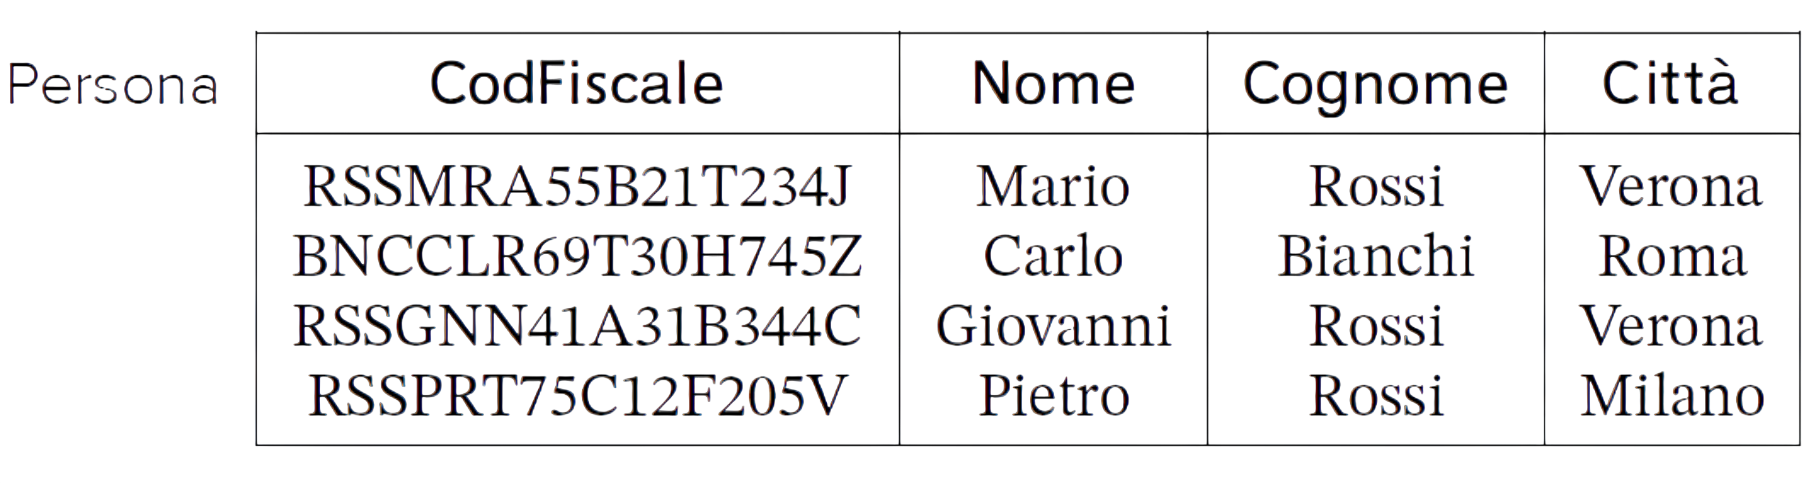
\includegraphics[width=0.6\textwidth]{images/tabella-persona.png}
  \end{center}

  \smallskip
  $\boldsymbol{\mathrm{Q_{10}}}$\textbf{: estrarre le città delle persone in cui il cognome è Rossi}
  \begin{lstlisting}[language=SQL]
  SELECT Citta
  FROM Persona
    WHERE Cognome = 'Rossi';
  \end{lstlisting}

  \smallskip
  L'output di questa interrogazione è la tabella:
  \begin{center}
    
\includegraphics[width=0.2\textwidth]{images/distinct-persona.png}
  \end{center}

  Per togliere i duplicati si può utilizzare la parola chiave $\verb|DISTINCT|$ dopo $\verb|SELECT|$:
  \begin{lstlisting}[language=SQL]
  SELECT DISTINCT Citta
  FROM Persona
    WHERE Cognome = 'Citta';
  \end{lstlisting}
  %foto
\end{esempiobox}

\section{Clausola \texttt{JOIN}}
In SQL, le interrogazioni con la clausola \verb|JOIN| si possono definire in due modi:
\begin{itemize}[label=$\triangleright$, itemsep=\smallskipamount]
  \item \textbf{senza l’uso di nuova sintassi}: specifica il legame tra le tabelle coinvolte a livello della clausola $\verb|WHERE|$
  \item \textbf{con l'uso di sintassi riservata} a livello di clausola $\verb|FROM|$
\end{itemize}

\smallskip
La clausola \verb|FROM| ammette come argomento:
\begin{lstlisting}[language=SQL]
  tabella [[AS] name] [, ...]
\end{lstlisting}

Si è visto che se sono presenti due o più nomi di tabelle, si esegue il prodotto cartesiano tra tutte le tabelle e lo schema del risultato
può contenere tutti gli attributi del prodotto cartesiano.\\[0.2ex]
Il prodotto cartesiano di due o più tabelle è un $\verb|CROSS JOIN|$.

\medskip
A partire da SQL-2, esistono altri tipi di \texttt{JOIN}:
\begin{itemize}[label=$\circ$, itemsep=\medskipamount]
  \item $\verb|INNER JOIN|$: restituisce solo le righe che soddisfano la condizione di join
  \item $\verb|LEFT [OUTER] JOIN|$: restituisce
  \begin{itemize}[label=$\diamond$, itemsep=\smallskipamount]
    \item tutte le righe della tabella di destra e sinistra che soddisfano la condizione di $\verb|join|$
    \item $\verb|null|$ per le righe della tabella di destra che non soddifisfano la condizione di di $\verb|join|$
  \end{itemize}
  \item $\verb|RIGH [OUTER] JOIN|$: restituisce
  \begin{itemize}[label=$\diamond$, itemsep=\smallskipamount]
    \item tutte le righe della tabella di destra e sinistra che soddisfano la condizione di $\verb|join|$
    \item $\verb|null|$ per le righe della tabella di sinistra che non soddifisfano la condizione di di $\verb|join|$
  \end{itemize}
  \item $\verb|FULL [OUTER] JOIN|$: restituisce
  \begin{itemize}[label=$\diamond$, itemsep=\smallskipamount]
    \item tutte le righe di entrambe le tabelle
    \item $\verb|null|$ per le righe che non soddifisfano la condizione di di $\verb|join|$
  \end{itemize}
\end{itemize}

In generale, la sintassi è:
\begin{lstlisting}[language=SQL]
tabella [NATURAL] join_type table_name [ ON condition [, ...]]
\end{lstlisting}

\begin{itemize}[label=$\triangleright$]
  \item $\verb|condition|$: espressione booleana che seleziona le tuple del $\verb|join|$ da aggiungere al risultato
\end{itemize}

\smallskip
Le tuple selezionate possono essere poi filtrate con la condizione della clausola $\verb|WHERE|$.

\begin{figure}[H]
  \centering
  \includegraphics[width=\textwidth]{images/Join.png}
\end{figure}

\subsection{Clausola \texttt{INNER JOIN}}
La sintassi è:
\begin{lstlisting}[language=SQL]
tabella [ INNER ] JOIN tabella ON join_condition [, ...]
\end{lstlisting}

Rappresenta il tradizionale $\theta$ $\verb|join|$ dell’algebra relazionale.\\[0.2ex]
Combina ciascuna riga $\mathrm{r_1}$ di $\mathrm{table_1}$ con ciascuna riga di $\mathrm{table_2}$ che soddisfa la condizione della clausola $\verb|ON|$.

\begin{esempiobox}{Interrogazione con \texttt{INNER JOIN}}
  \begin{lstlisting}[language=SQL]
  SELECT I.cognome, R.nomeRep, R.sede
  FROM Impiegato AS I
  INNER JOIN Reparto AS R ON I.nomeRep = R.nomeRep;
  \end{lstlisting}

  \begin{center}
    \includegraphics[width=0.5\textwidth]{images/tabellina.png}
  \end{center}
\end{esempiobox}

\subsection{Clausola \texttt{LEFT OUTER JOIN}}
La sintassi è:
\begin{lstlisting}[language=SQL]
tabella LEFT [ OUTER ] JOIN tabella ON join_condition [, ...]
\end{lstlisting}

Si esegue un $\verb|INNER JOIN|$.\\[0.2ex]
Poi, per ciascuna riga $\mathrm{r_1}$ di $\mathrm{table_1}$ che non soddisfa la condizione con qualsiasi riga di $\mathrm{table_2}$, si aggiunge una riga al risultato con i valori di $\mathrm{r_1}$ e assegnando $\verb|NULL|$ agli altri attributi.

\begin{esempiobox}{Interrogazione con \texttt{LEFT [OUTER] JOIN}}
  \begin{lstlisting}[language=SQL]
  INSERT INTO Reparto (nomerep, sede, telefono)
  VALUES ('Finanza', 'Padova', '02 8028888');

  SELECT R.nomeRep, I.cognome
  FROM Reparto AS R
  LEFT OUTER JOIN Impiegato AS I ON I.nomerep = R.nomerep;
  \end{lstlisting}

  \begin{center}
    \includegraphics[width=0.4\textwidth]{images/tabellina2.png}
  \end{center}
\end{esempiobox}

\vario{Nota}{
  Il $\texttt{LEFT OUTER JOIN}$ non è simmetrico!

  \smallskip
  Con le medisime tabelle si possono ottenere risultati diversi invertendo l’ordine delle tabelle nel join!
}

\subsection{Clausola \texttt{RIGHT OUTER JOIN}}
La sintassi è:
\begin{lstlisting}[language=SQL]
tabella RIGHT [ OUTER ] JOIN tabella ON join_condition [, ...]
\end{lstlisting}

\begin{esempiobox}{Interrogazione con \texttt{RIGHT [OUTER] JOIN}}
  \begin{lstlisting}[language=SQL]
  SELECT I.cognome , R.nomeRep
  FROM Impiegato I 
  RIGHT OUTER JOIN Reparto AS R ON I. nomerep = R. nomerep;
  \end{lstlisting}

  \begin{center}
    \includegraphics[width=0.5\textwidth]{images/tabellina2.png}
  \end{center}
\end{esempiobox}

\subsection{Clausola \texttt{FULL OUTER JOIN}}
La sintassi è:
\begin{lstlisting}[language=SQL]
tabella FULL [ OUTER ] JOIN tabella ON join_condition [, ...]
\end{lstlisting}

È equivalente a:
\begin{lstlisting}[language=SQL]
INNER JOIN + LEFT OUTER JOIN + RIGHT OUTER JOIN
\end{lstlisting}

Non è equivalente a $\verb|CROSS JOIN|$.

\section{Uso di variabili (alias)}
SQL permette di associare un nome alternativo (alias) alle tabelle che compaiono nella clausola $\verb|FROM|$.\\[0.2ex]
Il nome viene usato per far riferimento alla tabella nel contesto dell’interrogazione per diversi motivi:
\begin{itemize}[label=$\triangleright$, itemsep=\smallskipamount]
  \item far riferimento alla tabella in modo compatto
  \item fare accesso più volte alla stessa tabella
\end{itemize}

\begin{esempiobox}{Interrogazione con utilizzo di \texttt{AS}}
  Consideriamo la seguente tabella:

  \smallskip
  \begin{center}
    \includegraphics[width=0.6\textwidth]{images/tabella-impiegato.png  }
  \end{center}

  \smallskip
  $\boldsymbol{\mathrm{Q_{14}}}$\textbf{: estrarre tutti gli impiegati che hanno lo stesso cognome, ma nome diverso del dipartimento Produzione}
  \begin{lstlisting}[language=SQL]
  SELECT I1.Cognome, I2.Cognome
  FROM Impiegato I1, Impiegato I2
    WHERE I1.Cogmome = I2.Cognome AND
      I1.Nome <> I2.Cognome AND
      I2.Dipart = 'Produzione';
  \end{lstlisting}

  \smallskip
  Questa interrogazione confronta ciascuna riga di Impiegato con tutte le righe di Impiegato associate al dipartimento Produzione.

  \smallskip
  Si può immaginare che al momento della definizione dell’alias vengano create due copie della tabella Impiegato, ciascuna associata ad una delle due variabili $\mathrm{i_1}$ e $\mathrm{i_2}$.

  \smallskip
  Le due copie contengono tutte le righe di Impiegato.

  \smallskip
  Sulla copia $\mathrm{i_2}$ vengono selezionate solo le righe del dipartimento 'Produzione'.

  \smallskip
  \begin{center}
      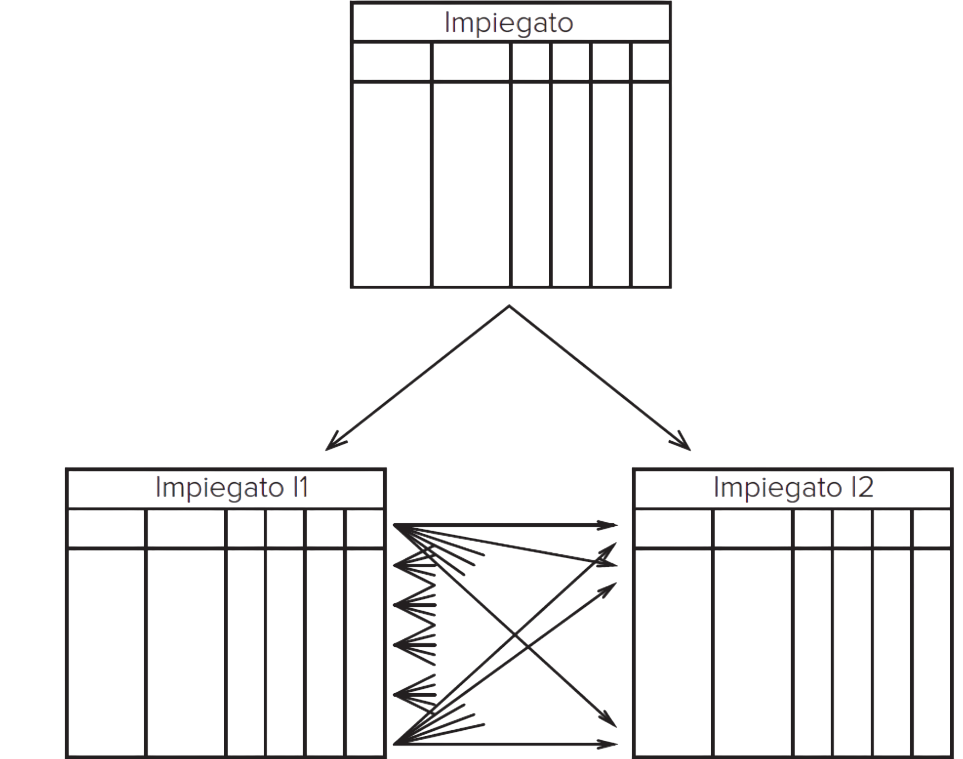
\includegraphics[width=0.4\textwidth]{images/Alias.png}
  \end{center}
\end{esempiobox}

\section{Clausola \texttt{ORDER BY}}
Una relazione è un insieme di tuple non ordinato, però, sorge spesso il bisogno di costruire un ordine sulle righe.\\[0.2ex]
SQL permette di specificare un ordinamento (ascendente o discendente) sulle righe dell‘output grazie alla clausola $\verb|ORDER BY|$ che chiude l‘interrogazione.

La sintassi è:
\begin{lstlisting}[language=SQL]
ORDER BY attributo [{ ASC | DESC }] [, ... ]
\end{lstlisting}

Le righe vengono ordinate per il primo attributo nell'elenco, a parità di valore del primo attributo si usa il secondo e così via in sequenza.

Di default l'ordinamento è $\verb|ASC|$.

\begin{esempiobox}{Interrogazione con \texttt{ORDER BY}}
  Consideriamo la seguente tabella:

  \smallskip
  \begin{center}
    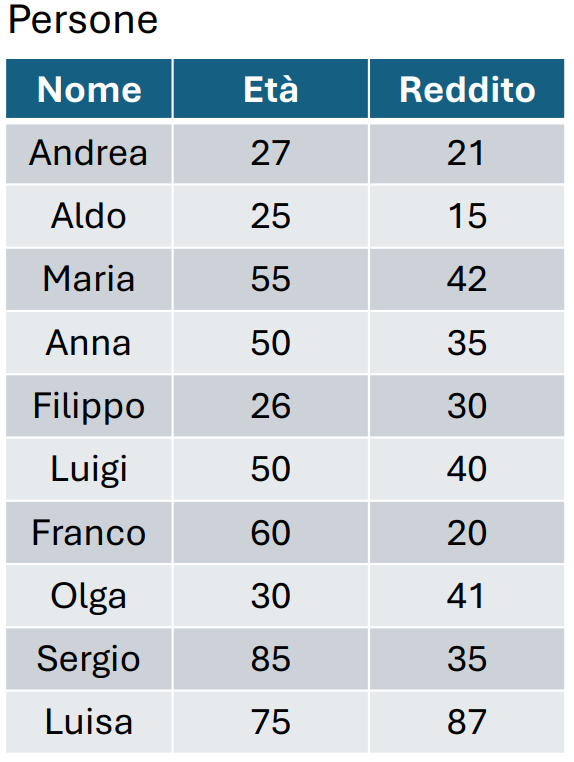
\includegraphics[width=0.3\textwidth]{images/tabella-persone.png}
  \end{center}

  \smallskip
  $\boldsymbol{\mathrm{Q_{15}}}$\textbf{: estrarre il nome, l'età e il reddito delle persone con meno di 30 anni in ordine alfabetico}

  \begin{lstlisting}[language=SQL]
  SELECT Nome, Eta, Reddito
  FROM Persone
    WHERE Eta < 30
      ORDER BY Eta;
  \end{lstlisting}
\end{esempiobox}

\begin{esempiobox}{Interrogazione con \texttt{ORDER BY}}
  Consideriamo la seguente tabella:

  \smallskip
  \begin{center}
    \includegraphics[width=0.5\textwidth]{images/Q11.png}
  \end{center}

  \smallskip
  $\boldsymbol{\mathrm{Q_{16}}}$\textbf{: estrarre il contenuto della tabella Automobile ordinato in base alla marca (discendente) e al modello}

  \begin{lstlisting}[language=SQL]
  SELECT *
  FROM Automobile
    ORDER BY Marca DESC, Modello;
  \end{lstlisting}
\end{esempiobox}

\section{Operazioni insiemistiche}
SQL mette a disposizione degli operatori insiemistci:
\begin{lstlisting}[language=SQL]
SELECT
  { UNION | INTERSECT | EXCEPT 
  [ALL] SELECT }
\end{lstlisting}

Gli operatori insiemistici, al contrario del resto del linguaggio, assumono come default di eseguire un'eliminazione dei duplicati, a meno che si usi $\verb|ALL|$.\\[0.2ex]
Sono sufficienti domini compatibili ed ugual numero di attributi.\\[0.2ex]
La corrispondenza si basa sulla posizione e se i nomi degli attributi sono diversi di solito il sistema usa il nome del primo operando.

\subsection{Unione}
\begin{esempiobox}{Interrogazione con unione}
  Consideriamo la seguente tabella:

  \smallskip
  \begin{center}
    \includegraphics[width=0.5\textwidth]{images/Q12.png}
  \end{center}

  \smallskip
  $\boldsymbol{\mathrm{Q}}$\textbf{: estrarre i nomi e i cognomi degli impiegati}

  \begin{lstlisting}[language=SQL]
  SELECT Nome
  FROM Impiegato
  UNION
  SELECT Cognome
  FROM Impiegato
  \end{lstlisting}
\end{esempiobox}

\begin{esempiobox}{Interrogazione con unione}
  Consideriamo la seguente tabella:

  \smallskip
  \begin{center}
    \includegraphics[width=0.5\textwidth]{images/Q13.png}
  \end{center}

  \smallskip
  $\boldsymbol{\mathrm{Q}}$\textbf{: etrarre i nomi e i cognomi degli impiegati eccetto quelli del dipartimento Amministrazione mantenendo i duplicati}

  \begin{lstlisting}[language=SQL]
  SELECT Nome
  FROM Impiegato
    WHERE Diaprt <> 'Amministrazione'
  UNION ALL
  SELECT Cognome
  FROM Impiegato
    WHERE Diaprt <> 'Amministrazione';
  \end{lstlisting}
\end{esempiobox}

\subsection{Intersezione}
\begin{esempiobox}{Interrogazione con intersezione}
  Consideriamo la seguente tabella:

  \smallskip
  \begin{center}
    \includegraphics[width=0.5\textwidth]{images/Q14.png}
  \end{center}

  \smallskip
  $\boldsymbol{\mathrm{Q}}$\textbf{: estrarre i cognomi degli impiegati che sono anche nomi}

  \begin{lstlisting}[language=SQL]
  SELECT Nome
  FROM Impiegato
  INTERSECT
  SELECT Cognome
  FROM Impiegato;
  \end{lstlisting}
\end{esempiobox}

\subsection{Differenza}
\begin{esempiobox}{Interrogazione con differenza}
  Consideriamo la seguente tabella:

  \smallskip
  \begin{center}
    \includegraphics[width=0.5\textwidth]{images/Q15.png}
  \end{center}

  \smallskip
  $\boldsymbol{\mathrm{Q}}$\textbf{: estrarre i nomi degli impiegati che non sono cognomi di qualche impiegato}

  \begin{lstlisting}[language=SQL]
  SELECT Nome
  FROM Impiegato
  EXCEPT
  SELECT Cognome
  FROM Impiegato;
  \end{lstlisting}
\end{esempiobox}

\section{Operatori aggregati}
Gli operatori di aggregazione permettono di valutare proprietà che dipendono da insiemi di tuple.

\subsection{Operatore \texttt{COUNT}}
L'operatore $\verb|COUNT|$ conta il numero di righe di una tabella o il numero di valori di uno o più attributi.

La sintassi è:
\begin{lstlisting}[language=SQL]
COUNT ( < * | [DISTINCT | ALL] ListaAttributi > )
\end{lstlisting}

\begin{itemize}[label=$\triangleright$, itemsep=\smallskipamount]
    \item $\verb|*|$: conta il numero di righe della tabella
    \item $\verb|DISTINCT ListaAttributi|$: conta il numero di valori diversi degli attributi ListaAttributi
    \item $\verb|ALL ListaAttributi|$: conta il numero di righe che hanno valori diversi da NULL negli attributi in ListaAttributi (default)
\end{itemize}

\begin{esempiobox}{Interrogazione con \texttt{COUNT}}
  Consideriamo la seguente tabella:

  \smallskip
  \begin{center}
    \includegraphics[width=0.5\textwidth]{images/Q16.png}
  \end{center}

  \smallskip
  $\boldsymbol{\mathrm{Q}}$\textbf{: estrarre il numero di impiegati del dipartimento di Produzione}
  \begin{lstlisting}[language=SQL]
  SELECT COUNT(*)
  FROM Impiegato
    WHERE Diaprt = 'Produzione';
  \end{lstlisting}
\end{esempiobox}

\begin{esempiobox}{Interrogazione con \texttt{COUNT}}
  Consideriamo la seguente tabella:

  \smallskip
  \begin{center}
    \includegraphics[width=0.5\textwidth]{images/Q17.png}
  \end{center}

  \smallskip
  $\boldsymbol{\mathrm{Q}}$\textbf{: estrarre il numero di valori diversi dell'attributo Stipendio fra tutte le righe di Impiegato}
  \begin{lstlisting}[language=SQL]
  SELECT COUNT(DISTINCT Stipendio)
  FROM Impiegato;
  \end{lstlisting}
\end{esempiobox}

\subsection{Operatore \texttt{SUM}}
L'operatore $\verb|SUM|$ estituisce la somma dei valori posseduti dall’espressione.

La sintassi è:
\begin{lstlisting}[language=SQL]
SUM ( < * | [DISTINCT | ALL] ListaAttributi > )
\end{lstlisting}

\begin{esempiobox}{Interrogazione con \texttt{SUM}}
  Consideriamo la seguente tabella:

  \smallskip
  \begin{center}
    \includegraphics[width=0.5\textwidth]{images/Q19.png}
  \end{center}

  \smallskip
  $\boldsymbol{\mathrm{Q}}$\textbf{: estrarre la somma degli stipendi del dipartimento Amministrazione}
  \begin{lstlisting}[language=SQL]
  SELECT SUM(Stipendio)
  FROM Impiegato
    WHERE Dipart = 'Amministrazione';
  \end{lstlisting}
\end{esempiobox}

\subsection{Operatore \texttt{MAX/MIN}}
Gli operatori $\verb|MIN|$ e $\verb|MAX|$ restituiscono rispettivamente il massimo e il minimo dei valori posseduti dall’espressione.

La sintassi è:
\begin{lstlisting}[language=SQL]
<MAX | MIN> ( [DISTINCT | ALL] ListaAttributi )
\end{lstlisting}

\subsection{Operatore \texttt{AVG}}
L'operatore $\verb|AVG|$ restiusce la media dei valori.

La sintassi è:
\begin{lstlisting}[language=SQL]
AVG ( [DISTINCT | ALL] ListaAttributi )
\end{lstlisting}

\begin{esempiobox}{Interrogazione con \texttt{MIN, MAX, AVG}}
  Consideriamo la seguente tabella:

  \smallskip
  \begin{center}
    \includegraphics[width=0.5\textwidth]{images/Q20.png}
  \end{center}

  \smallskip
  $\boldsymbol{\mathrm{Q}}$\textbf{: estrarre gli Stipendi minimi, massimi e medi fra quelli di tutti gli impiegati}
  \begin{lstlisting}[language=SQL]
  SELECT MIN(Stipendio), MAX(Stipendio), AVG(Stipendio)
  FROM Impiegato;
  \end{lstlisting}
\end{esempiobox}

\vario{Nota}{
  \begin{itemize}[label=$\triangleright$, itemsep=\smallskipamount]
  \item $\texttt{SUM}$ e $\texttt{AVG}$ ammettono come argomento solo espressioni che rappresentano valori numerici o intervalli di tempo
  \item $\texttt{MAX}$ e $\texttt{MIN}$ ammettono come argomento solo espressioni su cui è definito un ordinamento (quindi anche stringhe)
  \item $\texttt{DISTINCT}$ elimina i duplicati
  \item $\texttt{ALL}$ trascura solo i valori nulli
\end{itemize}
}

\begin{esempiobox}{ATTENZIONE}
  \begin{lstlisting}[language=SQL]
  SELECT Cognone, Nome, MAX(I.Stipendio)
  FROM Impiegato AS I
  JOIN Diparmento AS D ON I.Dipart = D.Nome
    WHERE D.Citta = 'Milano';
  \end{lstlisting}

  \textcolor{black!60!red}{\textbf{La seguente interrogazione non è corretta!}}
  
  \smallskip
  Gli operatori aggregati non sono un meccanismo di selezione, ma solo funzioni che restituiscono un valore quando sono applicate ad un insieme.

  \smallskip
  Cognome e Nome restituiscono un valore per ogni tupla selezionata, mentre $\texttt{MAX}$ restituisce un valore unico per tutto l’insieme.

  \smallskip
  Per risolvere questa situazione serve il meccanismo di \textbf{raggruppamento}.
\end{esempiobox}


\section{Clausola \texttt{GROUP BY}}
Gli operatori aggregate possono essere applicati separatamente a sottoinsiemi di righe.\\[0.2ex]
La clausola $\verb|GROUP BY|$ permette di specificare come dividere le tabelle in sottoinsiemi.\\[0.2ex]
La clausola permette di specificare un insieme di attributi e l’interrogazione raggrupperà le righe che possiedono gli stessi valori per questo insieme di attributi.

\begin{esempiobox}{Interrogazione con \texttt{GROUP BY}}
Consideriamo la seguente tabella:

\smallskip
\begin{center}
  \includegraphics[width=0.5\textwidth]{images/Q22.png}
\end{center}

\smallskip
$\boldsymbol{\mathrm{Q}}$\textbf{: estrarre la somma degli stipendi di tutti gli impiegati dallo stesso dipartimento}
\begin{lstlisting}[language=SQL]
SELECT Dipart, SUM(Stipendio)
FROM Impiegato
  GROUP BY Diaprt;
\end{lstlisting}
\end{esempiobox}

\smallskip
In una interrogazione che fa uso della clausola $\verb|GROUP BY|$ può comparire come argomento della $\verb|SELECT|$ solo un sottoinsieme degli attributi usati nella clausola $\verb|GROUP BY|$, oppure, operatori di aggregazione.

\subsection{Clausola \texttt{HAVING}}
È possibile applicare delle selezioni ai gruppi generati tramite la clausola $\verb|GROUP BY|$.\\[0.2ex]
La clausola $\verb|HAVING|$ permette di specificare delle condizioni che devono essere soddisfatte dai gruppi generati dopo l’esecuzione del raggruppamento tramite $\verb|GROUP BY|$.

La sintassi è:
\begin{lstlisting}[language=SQL]
SELECT Dipart, SUM(Stipendio) AS SommaStipendi
FROM Impiegato
  GROUP BY Dipart
    HAVING SUM(Stipendio) > 100;
\end{lstlisting}

Dopo aver eseguito i raggruppamenti, vengono mantenuti solo i gruppi che soddisfano la condizione specificata nella clausola $\verb|HAVING|$.

\begin{figure}[H]
\centering
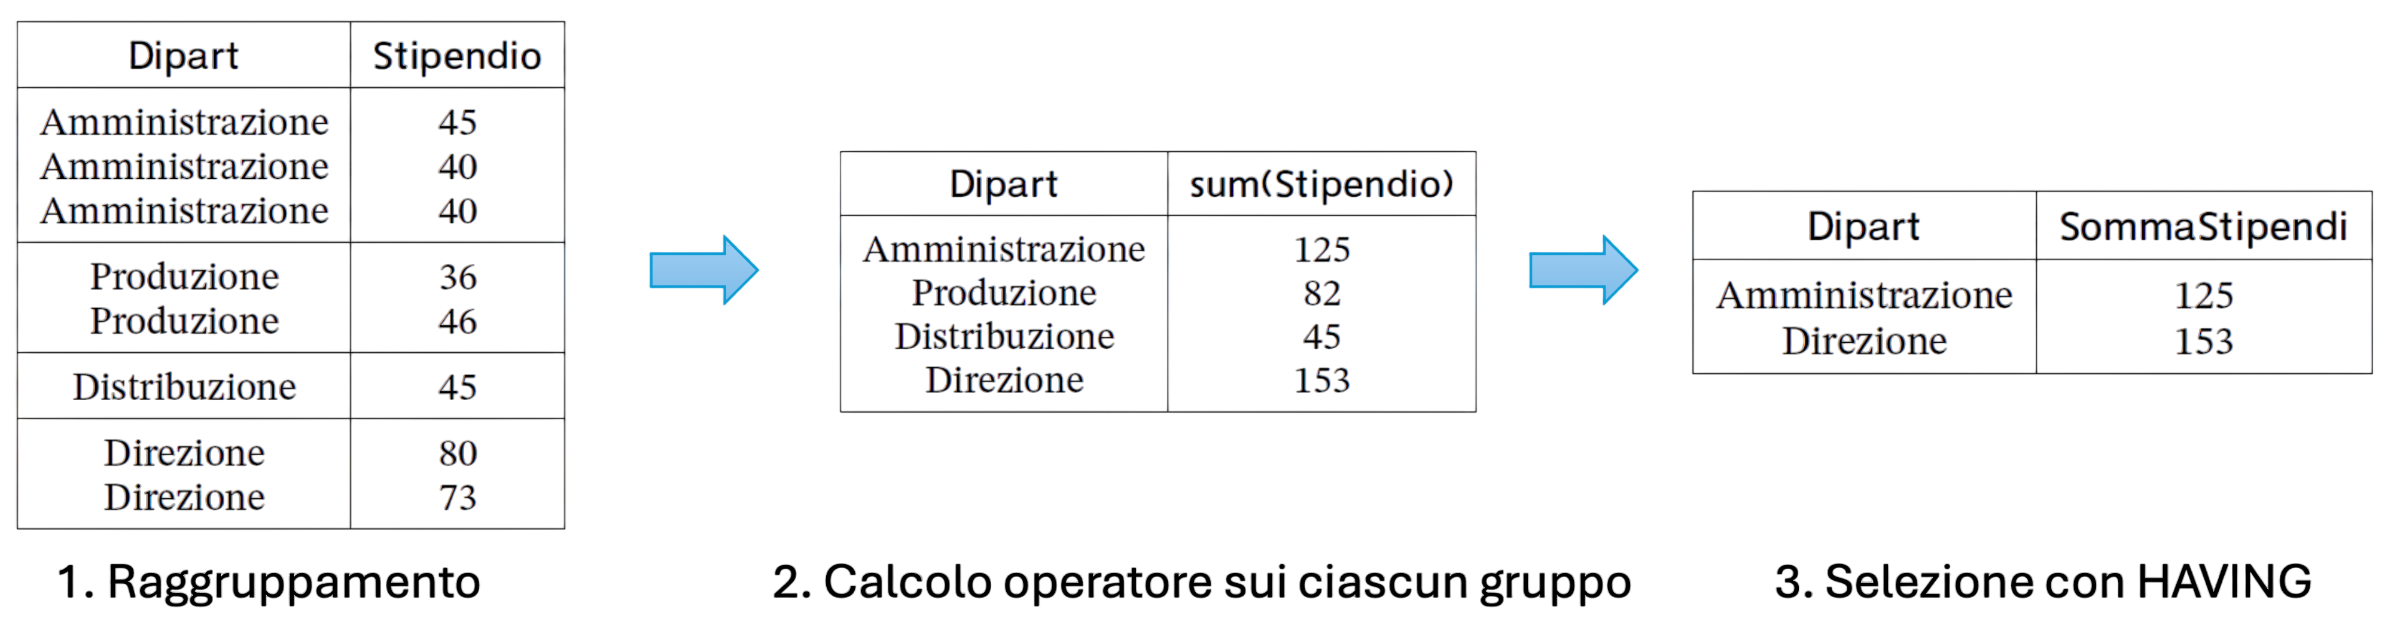
\includegraphics[width=\textwidth]{images/esempio.png}
\end{figure}

\begin{esempiobox}{OSSERVAZIONE}
\begin{itemize}[label=$\triangleright$, itemsep=\smallskipamount]
  \item clausola $\texttt{WHERE}$ applica delle selezioni su singole righe, \textcolor{purple}{\textbf{prima}} dell’eventuale raggruppamento tramite $\texttt{GROUP BY}$
  \item clausola $\texttt{HAVING}$ applica delle selezioni su gruppi, generati a \textcolor{purple}{\textbf{seguito}} dell’esecuzione del raggruppamento tramite $\texttt{GROUP BY}$
\end{itemize}

\begin{lstlisting}[language=SQL]
SELECT Dipart
FROM Impiegato
  WHERE Ufficio = 20 -- seleziona righe raggruppate
    GROUP BY Dipart  -- forma gruppi con righe selezionate
      HAVING AVG(Stipendio) > 25; -- seleziona gruppi del risultato
  \end{lstlisting}
\end{esempiobox}

\section{Interrogazioni nidificate}
Un' interrogazione nidificata è un'interrogazione che contiene al suo interno altre interrogazioni.\\[0.2ex]
La nidificazione può avvenire sia nella clausola $\verb|SELECT|$, che nella clausola $\verb|FROM|$, che nella clausola $\verb|WHERE|$.\\[0.2ex]
Il caso tipico è la nidificazione nella clausola $\verb|WHERE|$, dove un predicato contiene un confronto tra un valore (espressione su una singola riga) ed il risultato di un’interrogazione SQL.

\subsection{Clausola \texttt{WHERE}}
Se in un predicato si confronta un attributo o una espressione che produce un valore singolo con il risultato di un’interrogazione, sorge il problema di disomogeneità dei termini del confronto.\\[0.2ex]
I normali operatori di confronto ($\verb|=|, \verb|<>|, \verb|<|, \verb|>|, \verb|<=|, \verb|=>|$) possono essere estesi con le parole chiave $\verb|ANY|$ e $\verb|ALL|$:
\begin{itemize}[label=$\triangleright$, itemsep=\smallskipamount]
\item $\verb|ANY|$: riga soddisfa la condizione se risulta vero il confronto (con l’operatore specificato) tra il valore dell’attributo (o espressione) e \textbf{almeno} uno degli elementi restituiti dall’interrogazione 
\item $\verb|ALL|$: riga soddisfa la condizione se risulta vero il confronto (con l’operatore specificato) tra il valore dell’attributo (o espression) e \textbf{tutti} gli elementi restituiti dall’interrogazione
\end{itemize}

\begin{esempiobox}{Interrogazione con \texttt{WHERE}}
Consideriamo la seguente tabella:

\smallskip
\begin{center}
  \includegraphics[width=0.5\textwidth]{images/Q24.png}
\end{center}

\smallskip
$\boldsymbol{\mathrm{Q}}$\textbf{: estrarre i dipartimenti in cui non lavorano persone di cognome Rossi}
\begin{lstlisting}[language=SQL]
SELCET Nome
FROM Diparmento
  WHERE Nome <> ALL (
    SELECT Dipart
    FROM Impiegato
      WHERE Cognome = 'Rossi'
  );
\end{lstlisting}

\smallskip
Questo equivale a:
\begin{lstlisting}[language=SQL]
SELECT Nome
FROM Dipartimento
EXCEPT
SELECT Dipart
FROM Impiegato
WHERE Cognome = 'Rossi';
\end{lstlisting}
\end{esempiobox}

\vario{ATTENZIONE!}{
Per le interrogazioni nidificate viste fino ad ora, l’interrogazione può essere eseguita una volta sola ed il risultato ottenuto può essere salvato in una tabella temporanea usata per eseguire ciascun confronto con le righe dalla tabella esterna.

\smallskip
Talvolta però l’interrogazione nidificata fa riferimento al contesto dell’interrogazione che la racchiude attraverso l’uso di una variabile (\textbf{passaggio di binding}).

\smallskip
L’interrogazione nidificata dovrà essere \textbf{valutata separatamente per ciascuna riga} prodotta dalla valutazione della query esterna.
}

\subsection{Clausola \texttt{EXISTS}}
L'operatore logico $\verb|EXISTS|$ riceve come parametro un'interrogazione nidificata e restituisce il valore vero solo se l'interrogazione fornisce un risultato non vuoto.\\[0.2ex]
Questo operatore può essere usato in modo significativo soloquando si ha un passaggio di binding tra la query esterna e quella interna.

\begin{esempiobox}{Interrogazione con \texttt{EXISTS}}
Consideriamo la seguente tabella:

\smallskip
\begin{center}
  \includegraphics[width=0.5\textwidth]{images/Q25.png}
\end{center}

\smallskip
$\boldsymbol{\mathrm{Q}}$\textbf{: estrarre le persone che hanno degli omonimi (stesso nome e cognome, ma codice fiscale diverso)}
\begin{lstlisting}[language=SQL]
SELECT *
FROM Persona AS P
  WHERE EXISTS (
    SELECT *
    FROM Persona P1
    WHERE P1.Nome = P.Nome AND
      P1.Cognome = P.Cognome AND
      P1.CodFiscale <> P.CodFiscale
  );
\end{lstlisting}
\end{esempiobox}

\subsection{Clausola \texttt{SELECT}}
Le interrogazioni nidificate possono essere specificate anche come elemento della clausola $\verb|SELECT|$.

\vario{Nota}{
  Spesso l'uso di query nidificate nella \texttt{SELECT} sostituiscono l'uso del \texttt{JOIN}.
}

\begin{esempiobox}{Interrogazione con \texttt{SELECT}}
Consideriamo la seguente tabella:

\smallskip
\begin{center}
    \includegraphics[width=0.5\textwidth]{images/Q27.png}
\end{center}

\smallskip
$\boldsymbol{\mathrm{Q}}$\textbf{: estrarre per ogni cantante il numero di canzoni di cui è autore}
\begin{lstlisting}[language=SQL]
  SELECT DISTINCT Nome, NumCanzoni = (
    SELECT COUNT(*)
    FROM Autore AS A
      WHERE A.Nome = C.Nome
  )
  FROM Cantante AS C;
\end{lstlisting}
\end{esempiobox}


\subsection{Clausola \texttt{FROM}}
Le interrogazioni nidificate possono essere utilizzate nella clausola $\verb|FROM|$ come sorgente dati su cui eseguire l’interrogazione.\\[0.2ex]
È possibile creare una catena di interrogazioni, dove ciascuna interrogazione utilizza il risultato della precedente come una tabella di base.

\begin{esempiobox}{Interrogazione con \texttt{FROM}}
Consideriamo la seguente tabella:

\smallskip
\begin{center}
    \includegraphics[width=0.5\textwidth]{images/Q28.png}
\end{center}

\smallskip
$\boldsymbol{\mathrm{Q}}$\textbf{: estrarre per ogni cantante che è anche autore di canzoni il numero di canzoni di cui è rispettivamente interprete e autore}
\begin{lstlisting}[language=SQL]
SELECT DISTINCT C.Nome, C.NumCantate, A.NumScritte
FROM (
  SELECT Nome, COUNT(*) AS NumCantate
  FROM Cantante
) AS C
JOIN (
  SELECT Nome, COUNT(*) AS NumScritte
  FROM Autore
) AS A ON C.Nome = A.Nome;
\end{lstlisting}
\end{esempiobox}